\documentclass[
  shownotes,
  xcolor={svgnames},
  hyperref={colorlinks,citecolor=DarkBlue,linkcolor=DarkRed,urlcolor=DarkBlue}
  , aspectratio=169]{beamer}
\usepackage{animate}
\usepackage{amsmath}
\usepackage{amsfonts}
\usepackage{amssymb}
\usepackage{pifont}
\usepackage{mathpazo}
%\usepackage{xcolor}
\usepackage{multimedia}
\usepackage{fancybox}
\usepackage[para]{threeparttable}
\usepackage{multirow}
\setcounter{MaxMatrixCols}{30}
\usepackage{subcaption}
\usepackage{graphicx}
\usepackage{lscape}
\usepackage[compatibility=false,font=small]{caption}
\usepackage{booktabs}
\usepackage{ragged2e}
\usepackage{chronosys}
\usepackage{appendixnumberbeamer}
\usepackage{animate}
\setbeamertemplate{caption}[numbered]
\usepackage{color}
%\usepackage{times}
\usepackage{tikz}
\usepackage{comment} %to comment
%% BibTeX settings
\usepackage{natbib}
\bibliographystyle{apalike}
\bibpunct{(}{)}{,}{a}{,}{,}
\setbeamertemplate{bibliography item}{[\theenumiv]}

% Defines columns for bespoke tables
\usepackage{array}
\newcolumntype{L}[1]{>{\raggedright\let\newline\\\arraybackslash\hspace{0pt}}m{#1}}
\newcolumntype{C}[1]{>{\centering\let\newline\\\arraybackslash\hspace{0pt}}m{#1}}
\newcolumntype{R}[1]{>{\raggedleft\let\newline\\\arraybackslash\hspace{0pt}}m{#1}}


\usepackage{xfrac}


\usepackage{multicol}
\setlength{\columnsep}{0.5cm}

% Theme and colors
\usetheme{Boadilla}

% I use steel blue and a custom color palette. This defines it.
\definecolor{andesred}{HTML}{af2433}

% Other options
\providecommand{\U}[1]{\protect\rule{.1in}{.1in}}
\usefonttheme{serif}
\setbeamertemplate{itemize items}[default]
\setbeamertemplate{enumerate items}[square]
\setbeamertemplate{section in toc}[circle]

\makeatletter

\definecolor{mybackground}{HTML}{82CAFA}
\definecolor{myforeground}{HTML}{0000A0}

\setbeamercolor{normal text}{fg=black,bg=white}
\setbeamercolor{alerted text}{fg=red}
\setbeamercolor{example text}{fg=black}

\setbeamercolor{background canvas}{fg=myforeground, bg=white}
\setbeamercolor{background}{fg=myforeground, bg=mybackground}

\setbeamercolor{palette primary}{fg=black, bg=gray!30!white}
\setbeamercolor{palette secondary}{fg=black, bg=gray!20!white}
\setbeamercolor{palette tertiary}{fg=white, bg=andesred}

\setbeamercolor{frametitle}{fg=andesred}
\setbeamercolor{title}{fg=andesred}
\setbeamercolor{block title}{fg=andesred}
\setbeamercolor{itemize item}{fg=andesred}
\setbeamercolor{itemize subitem}{fg=andesred}
\setbeamercolor{itemize subsubitem}{fg=andesred}
\setbeamercolor{enumerate item}{fg=andesred}
\setbeamercolor{item projected}{bg=gray!30!white,fg=andesred}
\setbeamercolor{enumerate subitem}{fg=andesred}
\setbeamercolor{section number projected}{bg=gray!30!white,fg=andesred}
\setbeamercolor{section in toc}{fg=andesred}
\setbeamercolor{caption name}{fg=andesred}
\setbeamercolor{button}{bg=gray!30!white,fg=andesred}


\usepackage{fancyvrb}
\newcommand{\VerbBar}{|}
\newcommand{\VERB}{\Verb[commandchars=\\\{\}]}
\DefineVerbatimEnvironment{Highlighting}{Verbatim}{commandchars=\\\{\}}
% Add ',fontsize=\small' for more characters per line
\usepackage{framed}
\definecolor{shadecolor}{RGB}{248,248,248}
\newenvironment{Shaded}{\begin{snugshade}}{\end{snugshade}}
\newcommand{\AlertTok}[1]{\textcolor[rgb]{0.94,0.16,0.16}{#1}}
\newcommand{\AnnotationTok}[1]{\textcolor[rgb]{0.56,0.35,0.01}{\textbf{\textit{#1}}}}
\newcommand{\AttributeTok}[1]{\textcolor[rgb]{0.77,0.63,0.00}{#1}}
\newcommand{\BaseNTok}[1]{\textcolor[rgb]{0.00,0.00,0.81}{#1}}
\newcommand{\BuiltInTok}[1]{#1}
\newcommand{\CharTok}[1]{\textcolor[rgb]{0.31,0.60,0.02}{#1}}
\newcommand{\CommentTok}[1]{\textcolor[rgb]{0.56,0.35,0.01}{\textit{#1}}}
\newcommand{\CommentVarTok}[1]{\textcolor[rgb]{0.56,0.35,0.01}{\textbf{\textit{#1}}}}
\newcommand{\ConstantTok}[1]{\textcolor[rgb]{0.00,0.00,0.00}{#1}}
\newcommand{\ControlFlowTok}[1]{\textcolor[rgb]{0.13,0.29,0.53}{\textbf{#1}}}
\newcommand{\DataTypeTok}[1]{\textcolor[rgb]{0.13,0.29,0.53}{#1}}
\newcommand{\DecValTok}[1]{\textcolor[rgb]{0.00,0.00,0.81}{#1}}
\newcommand{\DocumentationTok}[1]{\textcolor[rgb]{0.56,0.35,0.01}{\textbf{\textit{#1}}}}
\newcommand{\ErrorTok}[1]{\textcolor[rgb]{0.64,0.00,0.00}{\textbf{#1}}}
\newcommand{\ExtensionTok}[1]{#1}
\newcommand{\FloatTok}[1]{\textcolor[rgb]{0.00,0.00,0.81}{#1}}
\newcommand{\FunctionTok}[1]{\textcolor[rgb]{0.00,0.00,0.00}{#1}}
\newcommand{\ImportTok}[1]{#1}
\newcommand{\InformationTok}[1]{\textcolor[rgb]{0.56,0.35,0.01}{\textbf{\textit{#1}}}}
\newcommand{\KeywordTok}[1]{\textcolor[rgb]{0.13,0.29,0.53}{\textbf{#1}}}
\newcommand{\NormalTok}[1]{#1}
\newcommand{\OperatorTok}[1]{\textcolor[rgb]{0.81,0.36,0.00}{\textbf{#1}}}
\newcommand{\OtherTok}[1]{\textcolor[rgb]{0.56,0.35,0.01}{#1}}
\newcommand{\PreprocessorTok}[1]{\textcolor[rgb]{0.56,0.35,0.01}{\textit{#1}}}
\newcommand{\RegionMarkerTok}[1]{#1}
\newcommand{\SpecialCharTok}[1]{\textcolor[rgb]{0.00,0.00,0.00}{#1}}
\newcommand{\SpecialStringTok}[1]{\textcolor[rgb]{0.31,0.60,0.02}{#1}}
\newcommand{\StringTok}[1]{\textcolor[rgb]{0.31,0.60,0.02}{#1}}
\newcommand{\VariableTok}[1]{\textcolor[rgb]{0.00,0.00,0.00}{#1}}
\newcommand{\VerbatimStringTok}[1]{\textcolor[rgb]{0.31,0.60,0.02}{#1}}
\newcommand{\WarningTok}[1]{\textcolor[rgb]{0.56,0.35,0.01}{\textbf{\textit{#1}}}}
\usepackage{graphicx}
\makeatletter

\definecolor{airforceblue}{rgb}{0.36, 0.54, 0.66}

\usepackage{tikz}
% Tikz settings optimized for causal graphs.
\usetikzlibrary{shapes,decorations,arrows,calc,arrows.meta,fit,positioning}
\tikzset{
    -Latex,auto,node distance =1 cm and 1 cm,semithick,
    state/.style ={ellipse, draw, minimum width = 0.7 cm},
    point/.style = {circle, draw, inner sep=0.04cm,fill,node contents={}},
    bidirected/.style={Latex-Latex,dashed},
    el/.style = {inner sep=2pt, align=left, sloped}
}


\makeatother






%%%%%%%%%%%%%%% BEGINS DOCUMENT %%%%%%%%%%%%%%%%%%

\begin{document}
 
\title[Lecture 25]{Lecture 25:  Boosting and Gradients}
\subtitle{Big Data and Machine Learning for Applied Economics \\ Econ 4676}
\date{\today}

\author[Sarmiento-Barbieri]{Ignacio Sarmiento-Barbieri}
\institute[Uniandes]{Universidad de los Andes}


\begin{frame}[noframenumbering]
\maketitle
\end{frame}

%%%%%%%%%%%%%%%%%%%%%%%%%%%%%%%%%%%




%----------------------------------------------------------------------% 

\begin{frame}
\frametitle{Agenda}

\tableofcontents

\end{frame}
%----------------------------------------------------------------------%
\section{Recap: Causal Trees}
%----------------------------------------------------------------------%
\begin{frame}[fragile]
\frametitle{Causal Trees for HTE}

\begin{itemize}
  \item Problem: we never observe $t_i$ unlike prediction that we observe $Y_i$
    \medskip
    \item Causal Trees search for leaves with
    \begin{itemize}
      \item HTE across leaves
      \medskip
      \item precisely-estimated leaf effects
    \end{itemize}
    \item Key is the honest Criterion
    \medskip
    \item Work well with RCTs
\end{itemize}


\end{frame}
%----------------------------------------------------------------------%
\section{Boosting: Motivation}
%----------------------------------------------------------------------%
\begin{frame}[fragile]
\frametitle{Boosting: Motivation}

\begin{itemize}

\item Boosting is one of the most powerful learning ideas introduced in the last twenty years. 

\item It was originally designed for classification problems, but  can  be extended to regression as well. 

\item The motivation for boosting was a procedure that combines the outputs of many “weak” classifiers to produce a powerful ensemble, “committee.” 


\item The idea of ensemble learning is to build a prediction model by combining the strengths of a collection of simpler base models.

\item  Bagging and random forests a committee of trees each cast a vote for the predicted class. 

\item Boosting is like as a committee method as well, although unlike random forests, the committee of weak learners evolves over time, and the members cast a weighted vote.


\end{itemize}

\end{frame}

%----------------------------------------------------------------------%
\section{Gradient-Based Optimization}
%----------------------------------------------------------------------%
\begin{frame}[fragile]
\frametitle{Detour: Gradient-Based Optimization}

\begin{itemize}
\item Most learning algorithms, especially learning, involve optimization of some sort. 
\medskip
\item Optimization refers to the task of either minimizing or maximizing some function $f(x)$ by altering $x$
\medskip
\item We usually phrase most optimization problems in terms of minimizing $f(x)$. 
\medskip
\item Maximization may be accomplished via a minimization algorithm by minimizing $-f(x)$.
\end{itemize}


\end{frame}
%----------------------------------------------------------------------%
\begin{frame}[fragile]
\frametitle{Detour: Gradient-Based Optimization}

\begin{itemize}
\item Suppose we have a function $y=f(x)$, where both x and y are real numbers.

\item The derivative $f'(x)$ gives the slope of $f(x)$ at the point x
\item  It specifies how to scale a small change in the input to obtain the corresponding change in the output

\begin{align}
f(x+\epsilon)\approx f(x)+\epsilon f'(x)
\end{align}

\item The derivative is therefore useful for minimizing a function because it tells us how to change x
in order to make a small improvement in y
\item  We can thus reduce $f(x)$ by moving x in small steps with the opposite sign of the derivative.
\item This technique is called gradient descent (Cauchy, 1847).

\end{itemize}

\end{frame}
%----------------------------------------------------------------------%
\begin{frame}[fragile]
\frametitle{Detour: Gradient-Based Optimization}



\begin{figure}[H] \centering
            \captionsetup{justification=centering}
              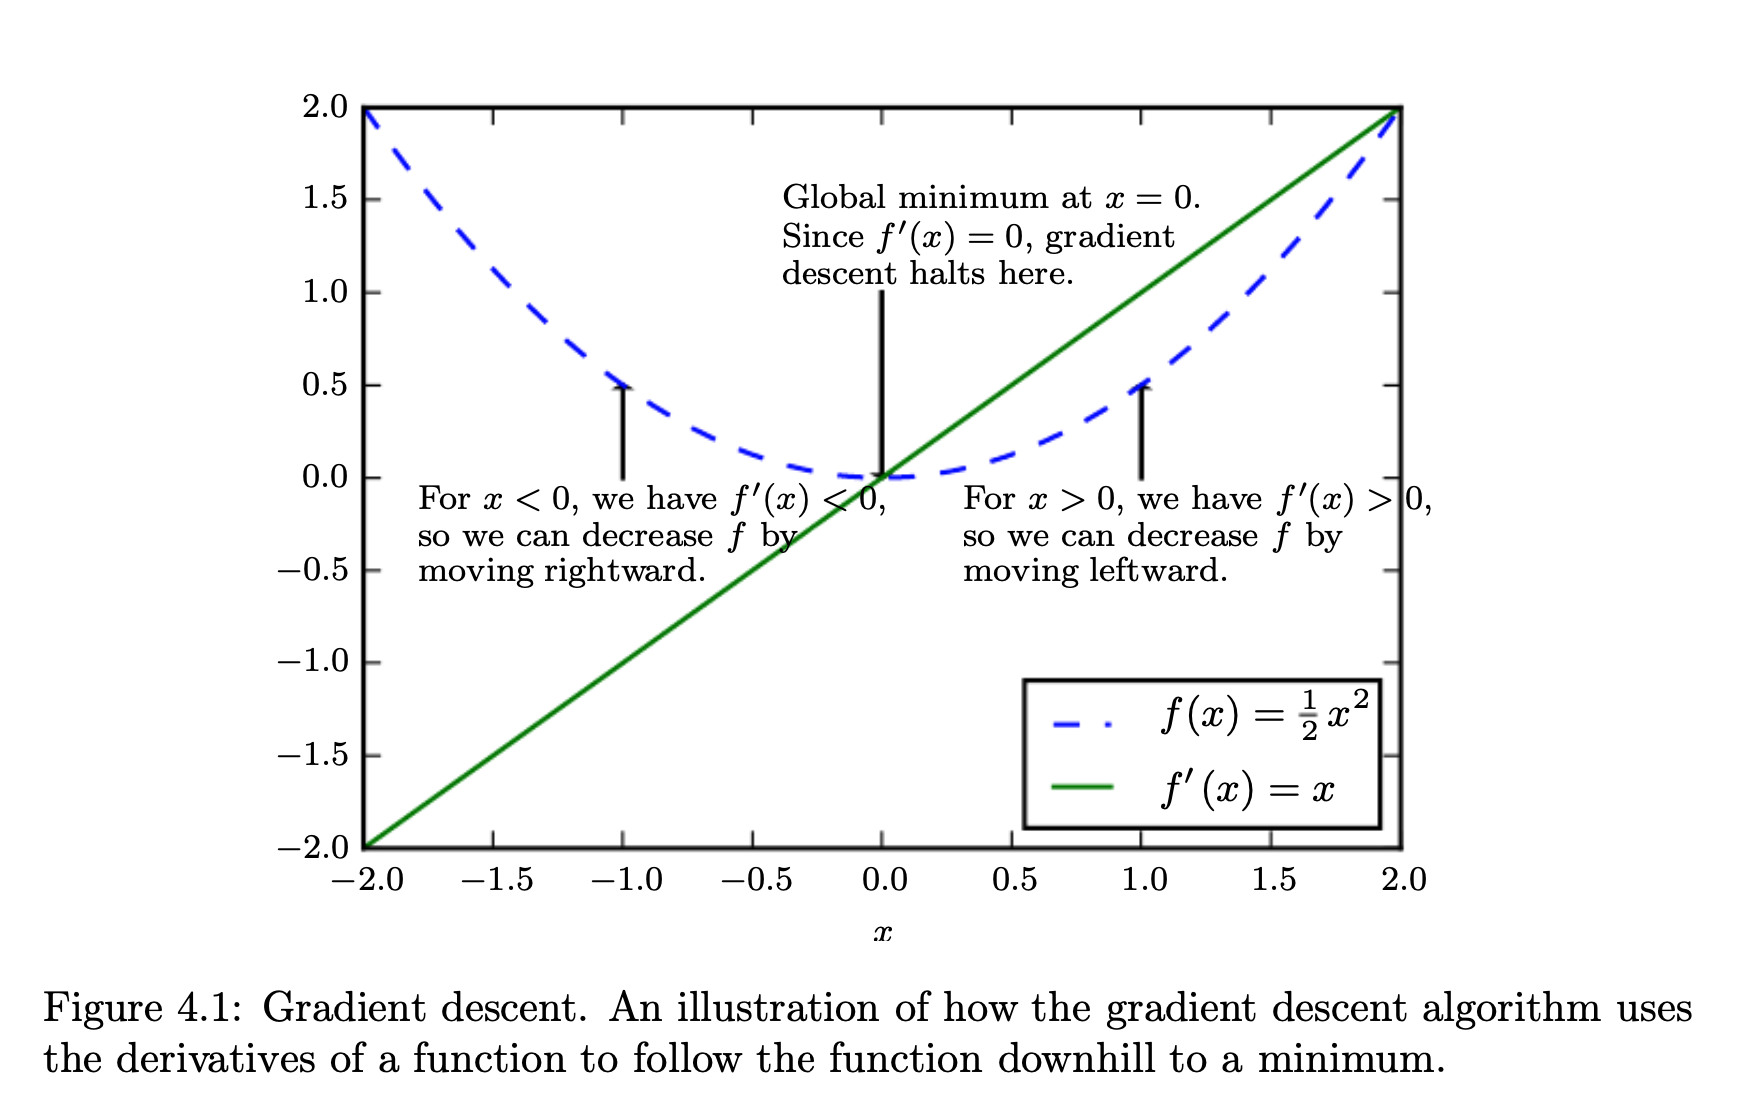
\includegraphics[scale=0.4]{figures/gradient_descent}
 \end{figure}
 \end{frame}
 %----------------------------------------------------------------------%
\begin{frame}[fragile]
\frametitle{Detour: Gradient-Based Optimization}



\begin{figure}[H] \centering
            \captionsetup{justification=centering}
              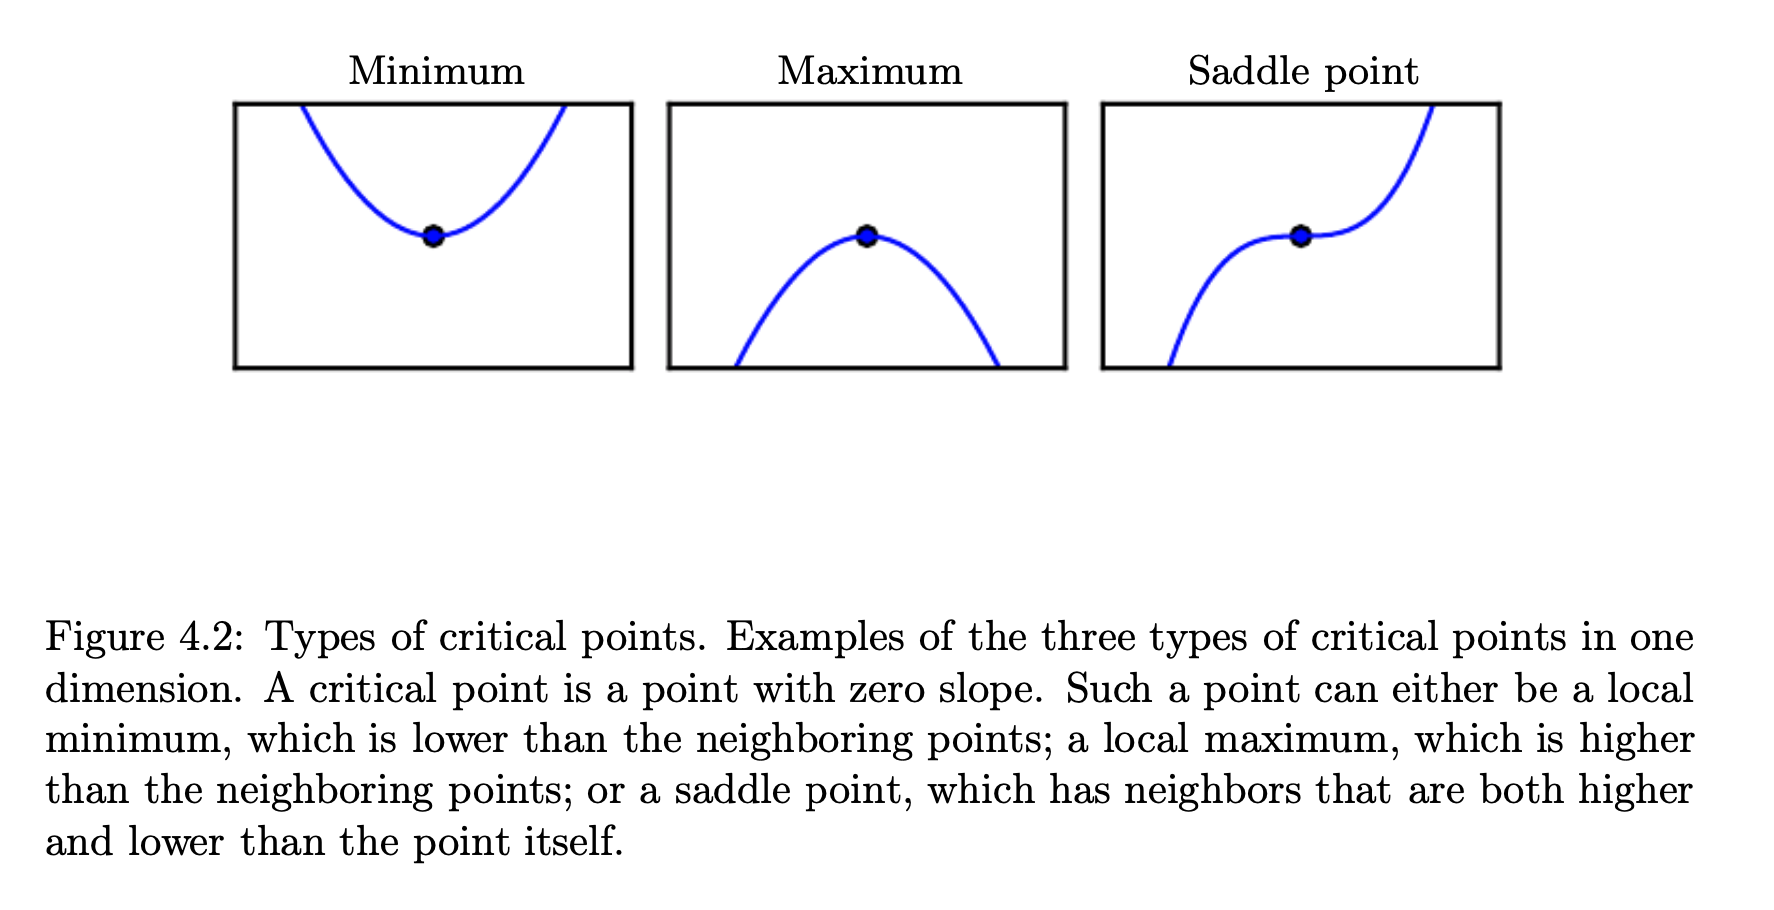
\includegraphics[scale=0.4]{figures/gradient_descent_2}
 \end{figure}
 
 \end{frame}
%----------------------------------------------------------------------%
\begin{frame}[fragile]
\frametitle{Detour: Gradient-Based Optimization}



\begin{figure}[H] \centering
            \captionsetup{justification=centering}
              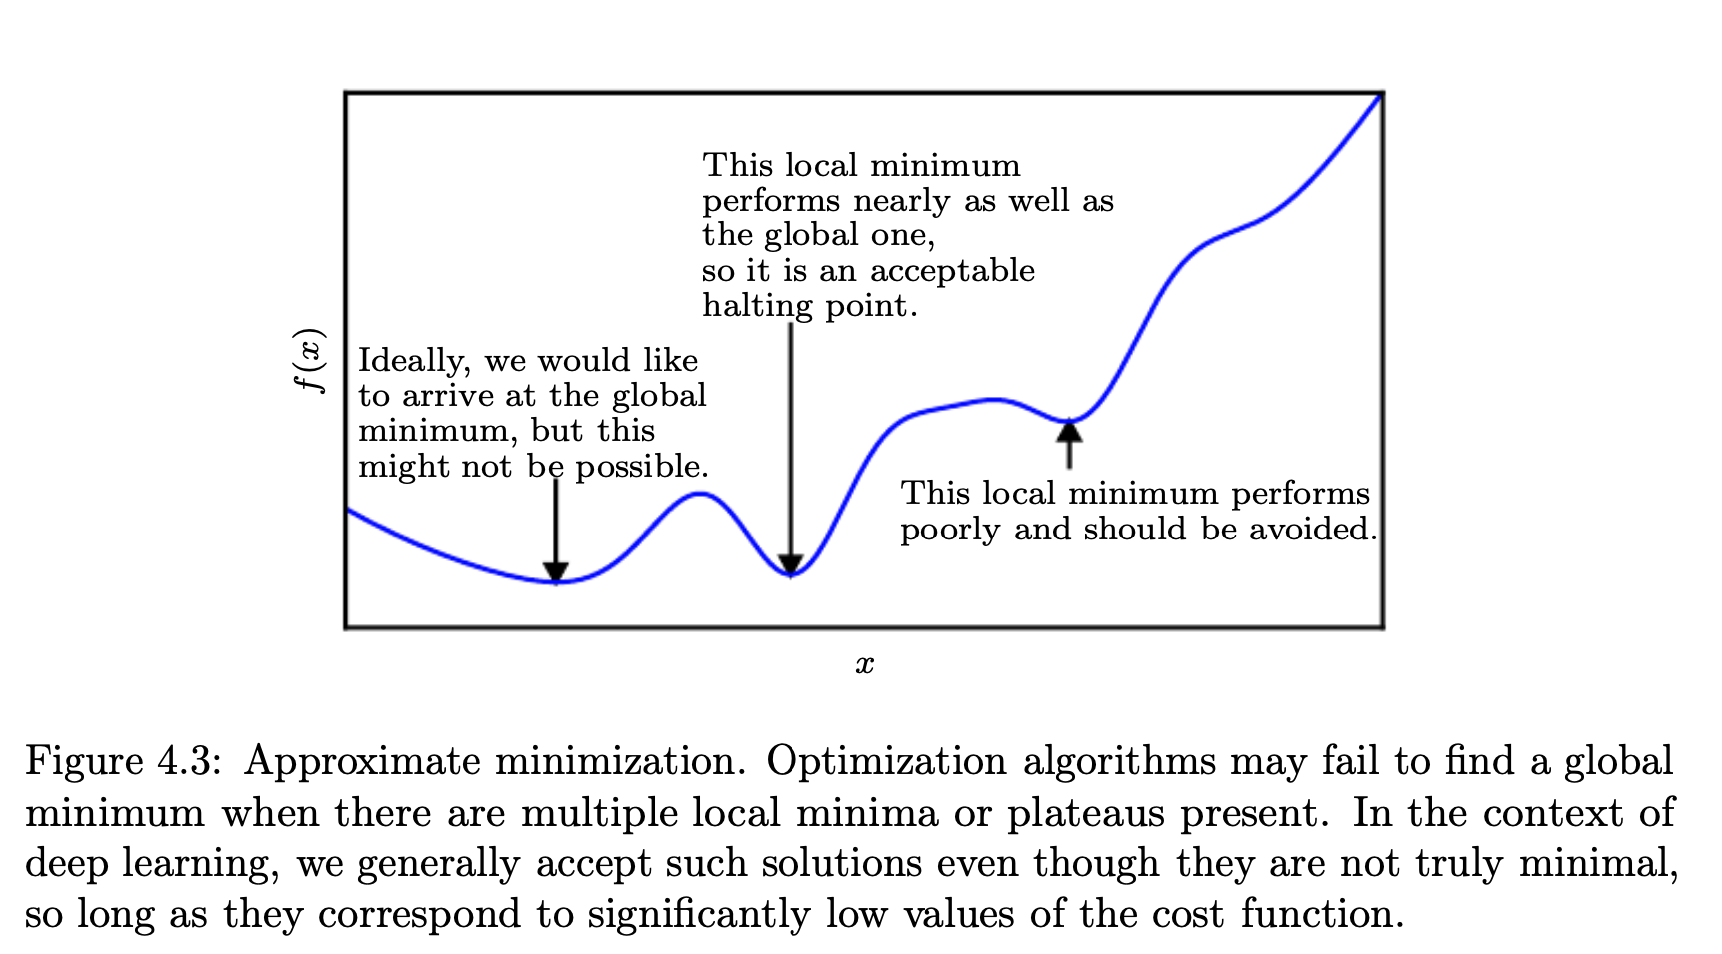
\includegraphics[scale=0.4]{figures/gradient_descent_3}
 \end{figure}
 
  \end{frame}
%----------------------------------------------------------------------%
\begin{frame}[fragile]
\frametitle{Detour: Gradient-Based Optimization}

\begin{itemize}


\item The directional derivative in direction $\mathbf{u}$ (a unit vector) is the slope of the function $f$ in direction $\mathbf{u}$. 
\item In other words, the directional derivative is the derivative of 
\begin{align}
f(x+\alpha u)
\end{align}
\item with respect to $\alpha$, evaluated at $\alpha=0$
\begin{align}
\frac{\partial}{\partial \alpha} = \mathbf{u}'\nabla_x f(\mathbf{u}) 
\end{align}
\end{itemize}

 
  \end{frame}
%----------------------------------------------------------------------%
\begin{frame}[fragile]
\frametitle{Detour: Gradient-Based Optimization}

\begin{itemize}
\item To minimize $f$, we would like to find the direction in which f decreases the fastest. 
\item We can use the directional derivative:

\begin{align}
\underset{u,u'u=1}{min}\mathbf{u}'\nabla_x f(\mathbf{u}) 
\end{align}
\begin{align}
\underset{u,u'u=1}{min}||\mathbf{u}||_2||\nabla_x f(\mathbf{u})||_2 \cos\,\theta 
\end{align}

\item Where $\theta$ is the angle between $\mathbf{u}$ and the gradient
\item Substituting $u'u=1$ 

\begin{align}
\underset{u,u'u=1}{min} \cos\,\theta 
\end{align}

\item This is minimized when $\mathbf{u}$ points in the opposite direction as the gradient.
\item In other words, the gradient points directly uphill, and the negative gradient points directly downhill.
\item We can decrease $f$ by moving in the direction of the negative gradient.
\item This is known as the method of {\bf steepest descent}, or {\bf gradient descent}

\end{itemize}

 
  \end{frame}
%----------------------------------------------------------------------%
\begin{frame}[fragile]
\frametitle{Detour: Gradient-Based Optimization}

\begin{itemize}
\item Steepest descent proposes a new point

\begin{align}
x'=x-\epsilon \nabla_x f(x)
\end{align}
\item where $\epsilon$ is the learning rate, a positive scalar determining the size of the step. 

\item We can choose $\epsilon$ in several different ways:
\begin{itemize}
\item A popular approach is to set $\epsilon$ to a small constant. 
 \item Sometimes, we can solve for the step size that makes the directional derivative vanish. 
 \item Another approach is to evaluate $f(x-\epsilon \nabla_x f(x))$ for several values of 
 $\epsilon$ and choose the one that results in the smallest objective function value. This  is called a line search.
\end{itemize}
 

\item Steepest descent converges when every element of the gradient is zero (or, in practice, very close to zero). 
\item In some cases, we may be able to avoid running this iterative algorithm and just jump directly to the critical point by solving the equation $\nabla_x f(x)=0$ for x.

\end{itemize}

 \end{frame}
%----------------------------------------------------------------------%
\section{Boosting}
 %----------------------------------------------------------------------%
\begin{frame}[fragile]
\frametitle{Boosting}

\begin{itemize}


\item The goal here is to solve something which looks like
\begin{align}
f^\star=\underset{f\in\mathcal{F}}{\text{argmin}}\left\lbrace \sum_{i=1}^n L(y_i,f(\mathbf{x}_i)) \right\rbrace
\end{align}


\item for some loss function $L$, and for some set of predictors $\mathcal{F}$. 

\item This is an optimization problem. 
\item Note that here in a function space, so we are solving for a function not a point.
\end{itemize}


\end{frame}
%----------------------------------------------------------------------%
\subsection{Boosting Trees}
%----------------------------------------------------------------------%
\begin{frame}[fragile]
\frametitle{Boosting Trees}

\begin{itemize}


\item In the case of trees, a constant is assigned to each region $(j=1,\dots,J)$ 
\item The predictive rule is
\begin{align}
x \in R_j\implies f(x)=c_j
\end{align}

\item A tree can be formally expressed as 
\begin{align}
T(x,\Omega)=\sum_{j=1}^K c_j I(x\in R_j)
\end{align}

\item with $\Omega=\{R_j,c_j\}^J_1$.
\item A Boosted tree model is a sum of trees
\begin{align}
f_M(x)=\sum_{m=1}^MT(x,\Omega_m)
\end{align}
\end{itemize}
 \end{frame}

%----------------------------------------------------------------------%
\begin{frame}[fragile]
\frametitle{Boosting Trees}
\framesubtitle{Numerical Optimization via Gradient Boosting}

\begin{itemize}
\item The objective is
\begin{align}
f^\star=\underset{f\in\mathcal{F}}{\text{argmin}}\left\lbrace \sum_{i=1}^n L(y_i,f(\mathbf{x}_i)) \right\rbrace
\end{align}

\item where $f(\mathbf{x}_i)(x)=\sum_{m=1}^MT(x,\Omega_m)$

\item Numerical optimization procedures solve $f^\star$ as a sum of component vectors

\begin{align}
f^\star_M=\sum_{m=0}^M h_m
\end{align}

\item $h_m\in \mathbb{R}^N$ where $f_0 =h_0$ is an initial guess and each successive $f_m$ is induced based on  the current parameter vector $f_{m-1}$, which is the sum of the previously induced updates. 
\item Numerical optimization methods differ in their prescriptions for computing each increment vector $h_m$ (“step”).
\end{itemize}

\end{frame}
%----------------------------------------------------------------------%
\begin{frame}[fragile]
\frametitle{Boosting Trees}
\framesubtitle{Implementations of Gradient Boosting}

\begin{itemize}
\item Gradient Tree Boosting Algorithm

\begin{enumerate}
\item Initialize $f_0(x)=\underset{c}{argmin}\sum_{i=1}^N L(y_i,c)$
\item for $m=1$ to $M$:
  \begin{enumerate}
      \item For $i=1,2,\dots N$ compute 
      \begin{align}
        r_{im}=-\left.\frac{\partial L(y_i,f(\mathbf{x}_i))}{\partial f(\mathbf{x}_i)}\right\vert_{f(\mathbf{x}_i)=f^{(m-1)}(\mathbf{x}_i)}
      \end{align}
      \item Fit a regression tree to the targets $r_{im}$ giving terminal regions $R_{jm}$ $j=1,2,\dots J_m$
      \item For $j=1,2,\dots,J_m$ compute
      \begin{align}
       c_{jm} =\underset{c}{argmin} \sum_{x_i\in R_{jm} } L(y_i,f_{m-1}(x_i)+c)
      \end{align}
      \item Update $f_m (x)=f_{(m-1)}(x) + \sum_{j=1}^{J_m} c_{jm} I(x \in R_{jm})$
  \end{enumerate}
  \item Output $\hat{f}(x)=f_M(x)$
\end{enumerate}


\end{itemize}

\end{frame}

%----------------------------------------------------------------------%
\subsection{Boosting Trees: Demo} 
%----------------------------------------------------------------------%
\begin{frame}[fragile]
\frametitle{Boosting Trees: Demo}
\begin{figure}[H] \centering
            \captionsetup{justification=centering}
              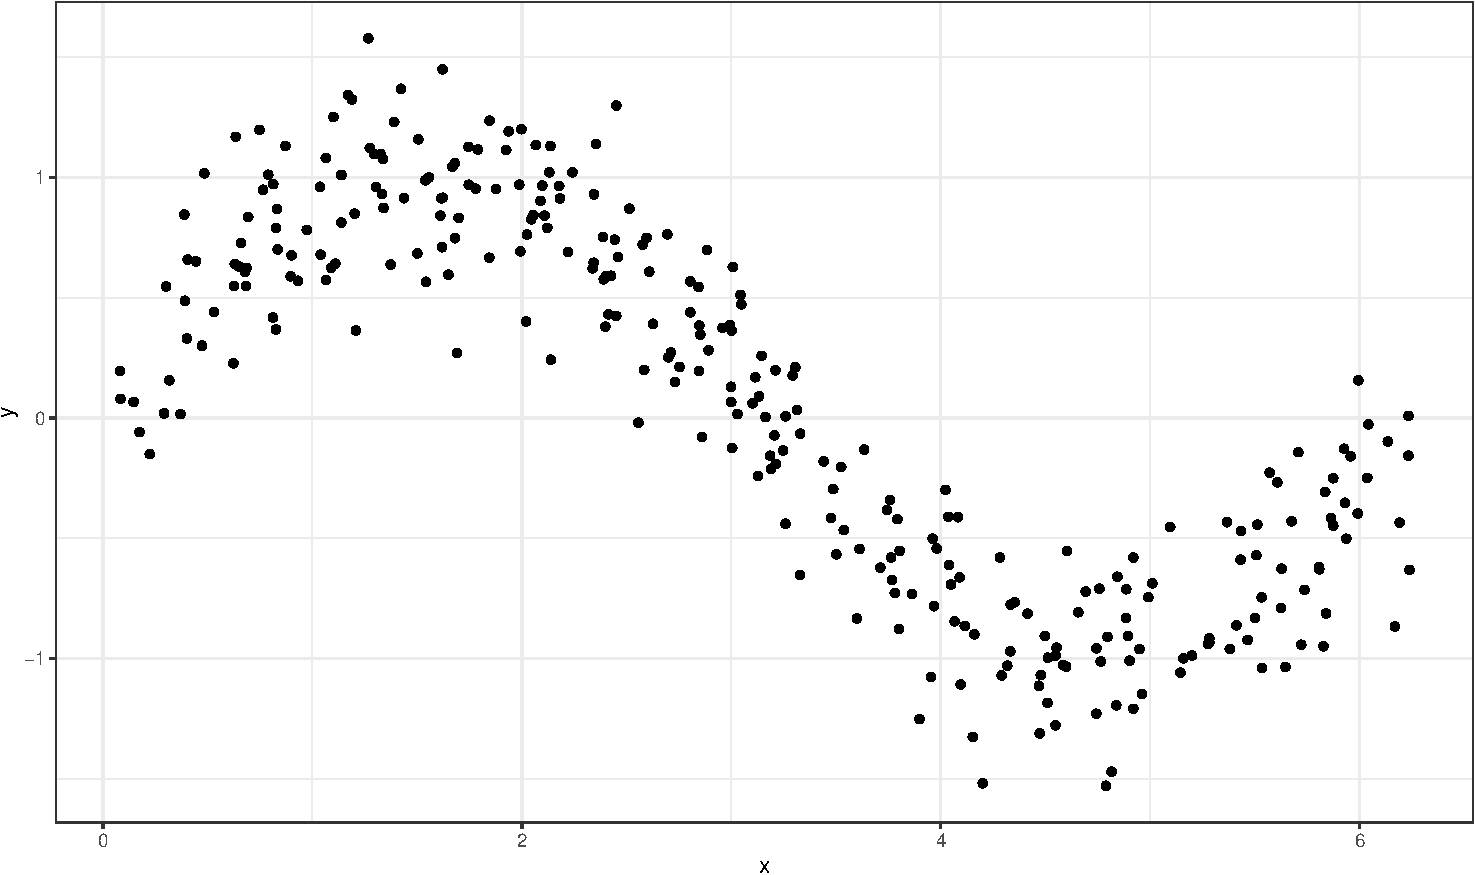
\includegraphics[scale=0.5]{figures/unnamed-chunk-3-1.pdf}
 \end{figure}


 \end{frame}
%----------------------------------------------------------------------%
\begin{frame}[fragile]
\frametitle{Boosting Trees: Example}

\begin{itemize}
\item Algorithm:
\end{itemize}

\begin{Shaded}
\begin{Highlighting}[]
\NormalTok{M\textless{}{-}}\DecValTok{2}
\end{Highlighting}
\end{Shaded}

\begin{figure}[H] \centering
            \captionsetup{justification=centering}
              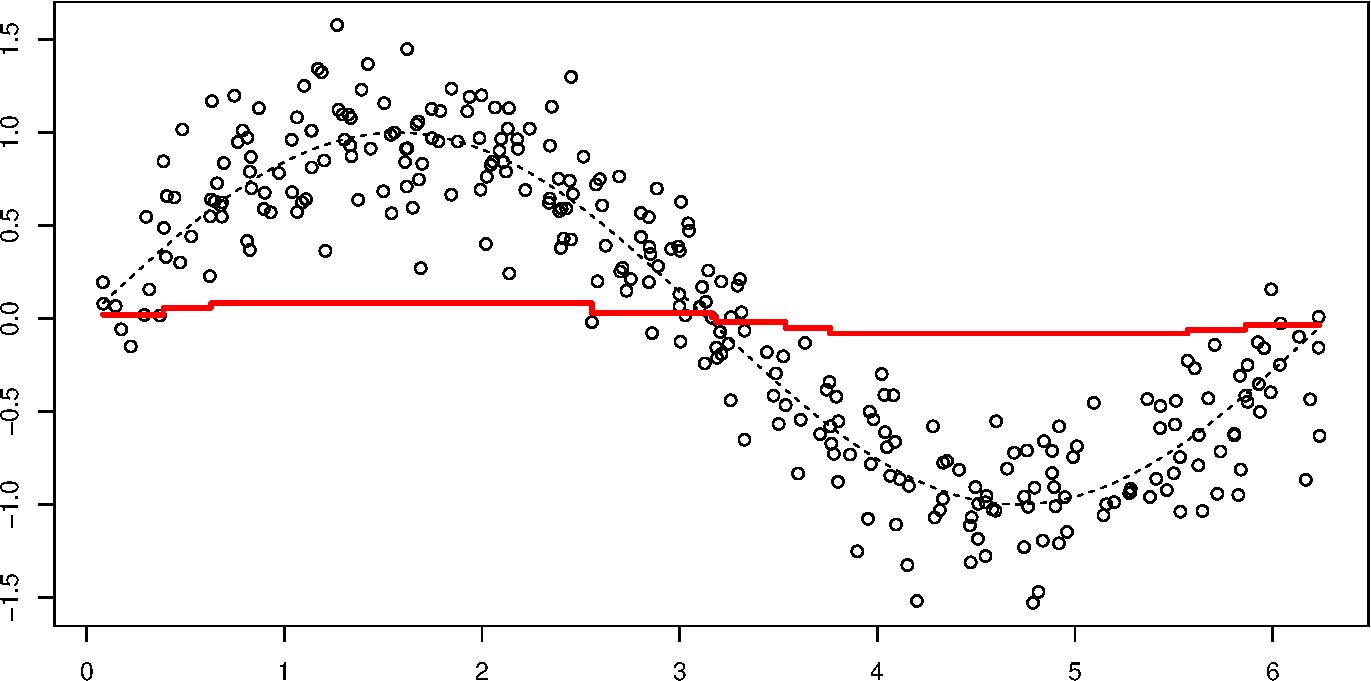
\includegraphics[scale=0.5]{figures/unnamed-chunk-5-1.pdf}
 \end{figure}

 \end{frame}
%----------------------------------------------------------------------%
\begin{frame}[fragile]
\frametitle{Boosting Trees: Example}

\begin{Shaded}
\begin{Highlighting}[]
\NormalTok{M\textless{}{-}}\DecValTok{10}
\end{Highlighting}
\end{Shaded}

\begin{figure}[H] \centering
            \captionsetup{justification=centering}
              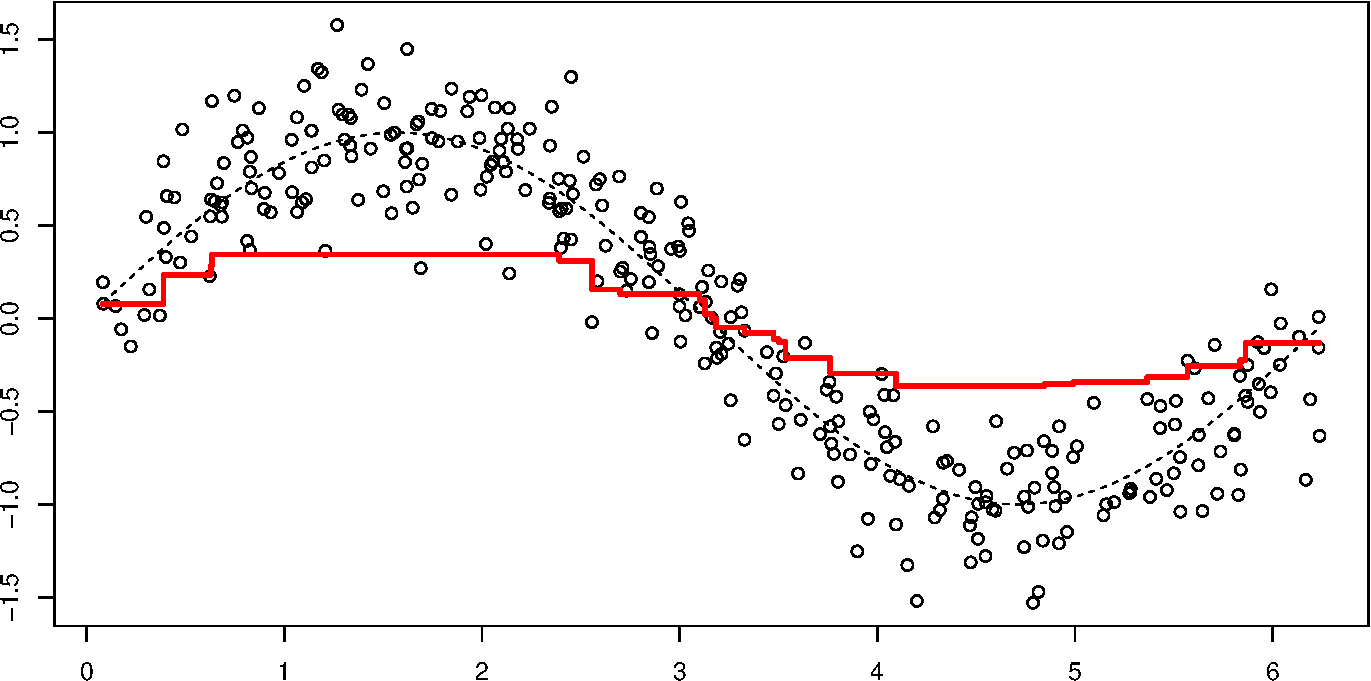
\includegraphics[scale=0.5]{figures/unnamed-chunk-6-1.pdf}
 \end{figure}
 \end{frame}
%----------------------------------------------------------------------%
\begin{frame}[fragile]
\frametitle{Boosting Trees: Example}

\begin{Shaded}
\begin{Highlighting}[]
\NormalTok{M\textless{}{-}}\DecValTok{100}
\end{Highlighting}
\end{Shaded}

\begin{figure}[H] \centering
            \captionsetup{justification=centering}
              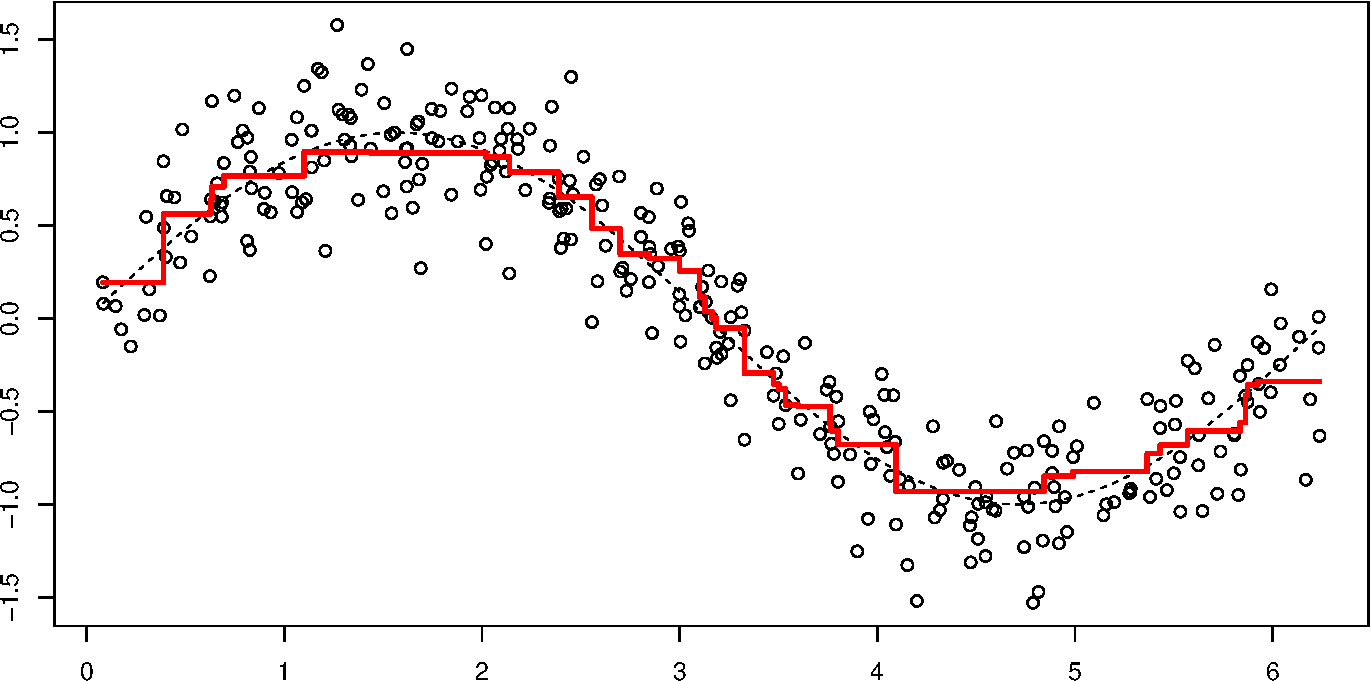
\includegraphics[scale=0.5]{figures/unnamed-chunk-7-1.pdf}
 \end{figure}

 \end{frame}
%----------------------------------------------------------------------%
\begin{frame}[fragile]
\frametitle{Boosting Trees: Example}

\begin{Shaded}
\begin{Highlighting}[]
\NormalTok{M\textless{}{-}}\DecValTok{300}

\end{Highlighting}
\end{Shaded}

\begin{figure}[H] \centering
            \captionsetup{justification=centering}
              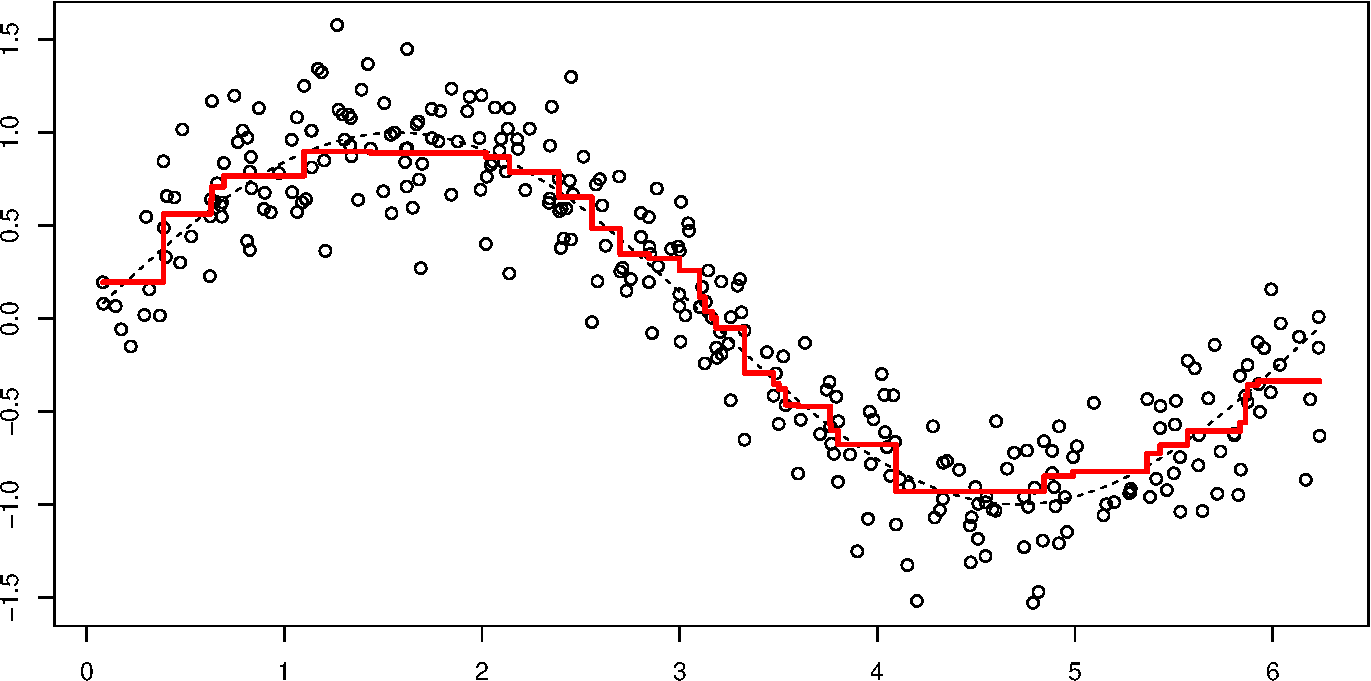
\includegraphics[scale=0.5]{figures/unnamed-chunk-8-1.pdf}
 \end{figure}

 \end{frame}
%----------------------------------------------------------------------%
\begin{frame}[fragile]
\frametitle{Boosting Trees: Example}

\begin{itemize}
\item Simple tree (blue), boosted tree (red)
\end{itemize}

\begin{figure}[H] \centering
            \captionsetup{justification=centering}
              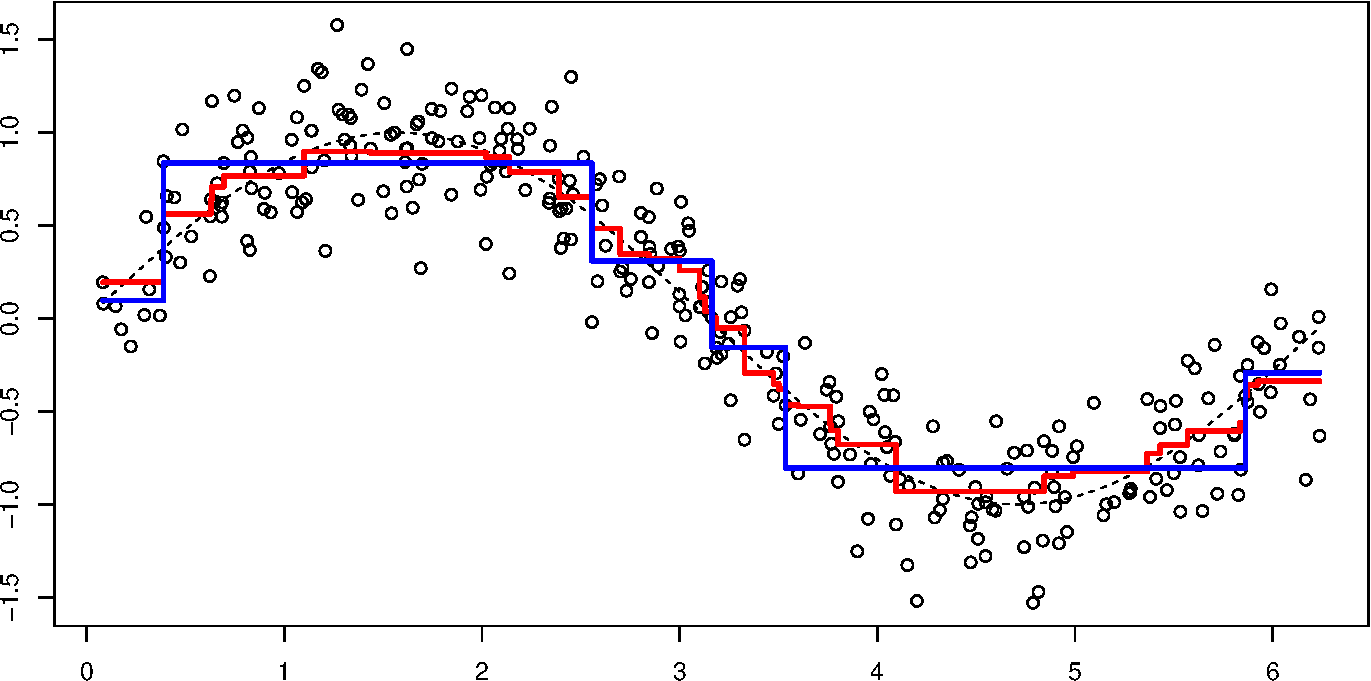
\includegraphics[scale=0.5]{figures/unnamed-chunk-9-1.pdf}
 \end{figure}

 \end{frame}
%----------------------------------------------------------------------%
\begin{frame}[fragile]
\frametitle{Boosting Trees: Algorithm explained}

\begin{itemize}
\item Learning tree structure is much harder than traditional optimization problem where you can simply take the gradient. 
\item It is intractable to learn all the trees at once. 
\item Instead, we use an additive strategy: fix what we have learned, and add one new tree at a time. We write the prediction value at step m as $\hat{y}_i^{m}$. 
\item Then we have
\begin{align}
\hat{y}_i^{0} &=0 \\ \nonumber
\hat{y}_i^{1} &= \hat{y}_i^{1} + f_1(x_i) \\ \nonumber
\hat{y}_i^{2} &= \hat{y}_i^{2} + f_2(x_i) \\ \nonumber
\dots \\ \nonumber
\hat{y}_i^{M} &= \sum_{m=1}^M f_m(x_i) = \hat{y}_i^{m-1} + f_m(x_i) \\ \nonumber
\end{align}
\end{itemize}


 \end{frame}
%----------------------------------------------------------------------%
\begin{frame}[fragile]
\frametitle{Boosting Trees: Algorithm explained}

\begin{itemize}


\item Which tree do we want at each step? 
\item Add the one that optimizes our objective.

\begin{align}
obj^m &= \sum_{i=1}^N L(y_i,\hat{y}_i^{(m)}) \\
     &= \sum_{i=1}^N L(y_i,\hat{y}_i^{m-1} + f_m(x_i))
\end{align}

\item If we consider using mean squared error (MSE) as our loss function, the objective becomes

\begin{align}
\sum_{i=1}^N (y_i-\hat{y}_i^{m-1} + f_m(x_i))^2
\end{align}

\item  For other losses of interest (for example, logistic loss), it is not so easy to get such a nice form.
\end{itemize}
 \end{frame}
%----------------------------------------------------------------------%
\begin{frame}[fragile]
\frametitle{Boosting Trees: Algorithm explained}

\begin{itemize}
\item  So in the general case, we take the Taylor expansion of the loss function:

\begin{align}
obj^m &= \sum_{i=1}^N \left[ L(y_i,\hat{y}_i^{(m)}) + r_{im} f_m(x_i) \right]
\end{align}

where 

\begin{align}
        r_{im}=-\left.\frac{\partial L(y_i,f(\mathbf{x}_i))}{\partial f(\mathbf{x}_i)}\right\vert_{f(\mathbf{x}_i)=f^{(m-1)}(\mathbf{x}_i)}
  \end{align}

\item After we remove all the constants, the specific objective at step m becomes


\begin{align}
obj^m &= \sum_{i=1}^N \left[ r_{im} f_m(x_i) \right]
\end{align}

\item This becomes our optimization goal for the new tree. One important advantage of this definition is that the value of the objective function only depends on $r_i$ 
\end{itemize}
 \end{frame}
%----------------------------------------------------------------------%
\begin{frame}[fragile]
\frametitle{Boosting Trees: Regularization}

\begin{itemize}

\item How many iterations (M)?
\begin{itemize}
\medskip

\item Each iteration usually reduces the training risk $L(.)$, so that for M large enough this risk
can be made arbitrarily small.
\medskip
\item  However, fitting the training data too well can lead to overfitting, which degrades the risk on future predictions. 
\medskip
\item Thus, there is an optimal number $M^\star$ minimizing future risk that is application dependent. 
\medskip
\item A convenient way to estimate $M^\star$ is to monitor prediction risk as a function of M on a validation sample. The value of M that minimizes  this risk is taken to be an estimate of M . 
\end{itemize}
\end{itemize}
\end{frame}

%----------------------------------------------------------------------%
\begin{frame}[fragile]
\frametitle{Boosting Trees: Regularization}
\begin{itemize}
\item Shrinkage
\begin{itemize}
  \item The simplest implementation of shrinkage in the context of boosting is to scale the contribution of each tree by a factor $\nu \in (0,1)$ when it is added to the current approximation. That is, we replace step 
  \begin{align}
   \hat{y}_m (x)=f_{(m-1)}(x) + \nu f_m(x_i)
  \end{align}
  \item Empirically it has been found  that smaller values of $\nu$ favor better test error, and require correspondingly larger values of $M$. 
  \item the best strategy appears to be to set $\nu$ to be very small ($\nu < 0.1$)
  \item This yields dramatic improvements (over no shrinkage $\nu$ = 1) 
\end{itemize} 
\item Subsampling
\begin{itemize}
\item With stochastic gradient boosting, at each iteration we sample a fraction $\eta$ of the training observations (without replacement), and grow the next tree using that subsample. 
\item Reduces the computing time by the same fraction $\eta$, and some cases improves prediction
\end{itemize}
\end{itemize}

\end{frame}
%----------------------------------------------------------------------%
\section{XGBoost: Next Class Preview}
%----------------------------------------------------------------------%
\begin{frame}[fragile]
\frametitle{XGBoost: Next Class Preview}

\begin{itemize}


\item Now that you understand decision trees and gradient boosting, understanding XGBoost becomes easy: it is a gradient boosting algorithm that uses decision trees 
\item Beyond that, its implementation was specifically engineered for optimal performance and speed.



\item Why talk about XGBoost?
\begin{itemize}


 \item Among the 29 challenge winning solutions published in Kaggle's blog during 2015, 17 solutions used XGBoost.  
 \item Among these solutions,  eight  solely  used  XGBoost  to  train  the  model, while most others combined XGBoost with neural nets in ensembles. (The second most popular method, deep  neural  nets,  was  used  in  11  solutions) 
 \item   The  success of the system was also witnessed in 2015 Data Mining and Knowledge Discovery competition organized by ACM (KDD Cup) , where XGBoost  was  used  by  every  winning  team  in  the  top-10. 
 \item Historically, XGBoost has performed quite well for structured, tabular data. But, if you are dealing with non-structured data such as images, neural networks are usually a better option (more on this later)
\end{itemize}
 \end{itemize}
\end{frame}






%----------------------------------------------------------------------%
%----------------------------------------------------------------------%
\section{Review
 \& Next Steps}
%----------------------------------------------------------------------%
\begin{frame}
\frametitle{Review \& Next Steps}
  
\begin{itemize} 
    \item Gradient Based Optimization
    \medskip
    \item Boosting Trees
    \begin{itemize}
      \item How it works
    \end{itemize}
    \item Preview next class: XGBOOST
    \medskip  
    \item Questions? Questions about software? 

\end{itemize}
\end{frame}
%----------------------------------------------------------------------%
\section{Further Readings}
%----------------------------------------------------------------------%
\begin{frame}
\frametitle{Further Readings}

\begin{itemize}

  \item Charpentier, Arthur (2018). Classification from scratch, boosting. \url{https://freakonometrics.hypotheses.org/tag/xgboost}
  \medskip
  \item Chen, T., \& Guestrin, C. (2016, August). Xgboost: A scalable tree boosting system. In Proceedings of the 22nd acm sigkdd international conference on knowledge discovery and data mining (pp. 785-794).
  \medskip
  \item Friedman, J., Hastie, T., \& Tibshirani, R. (2001). The elements of statistical learning (Vol. 1, No. 10). New York: Springer series in statistics.
  \medskip
  \medskip Goodfellow, I., Bengio, Y., Courville, A., \& Bengio, Y. (2016). Deep learning. Cambridge: MIT press.

  
\end{itemize}

\end{frame}





%----------------------------------------------------------------------%
%----------------------------------------------------------------------%
\end{document}
%----------------------------------------------------------------------%
%----------------------------------------------------------------------%

